\chapter{General implications}

We will be interested in seeing which laws imply which other laws, in the sense that magmas obeying the former law automatically obey the latter.  We will also be interested in \emph{anti-implications} showing that one law does \emph{not} imply another, by producing examples of magmas that obey the former law but not the latter. Here is a formal definition.

\begin{definition}[Implication]\label{impl}\uses{models-def}  A law $E$ is said to \emph{imply} another law $E'$ if $\{E\} \models E'$, or equivalently:
  $$ G \models w  \formaleq  w' \implies G \models w''  \formaleq  w''' \hbox{ for all magmas } G$$
Two laws are said to be \emph{equivalent} if they imply each other.
\end{definition}

\begin{lemma}[Pre-order]\leanok\label{pre-order}\uses{impl}  If we define $E \leq E'$ if $E$ implies $E'$, then this is a pre-order on the set of laws, and equivalence is an equivalence relation.
\end{lemma}

Note that we view the stronger law as less than or equal to the weaker law.  This is because the class of magmas that obey the stronger law is a subset of the class of magmas that obey the weaker law.  It is also consistent with the conventions of Lean's Mathlib.

\begin{proof}\leanok Trivial.
\end{proof}

Implications between the laws from Chapter \ref{subgraph-eq} are depicted in Figure \ref{fig:implications}.

\begin{figure}
  \centering
  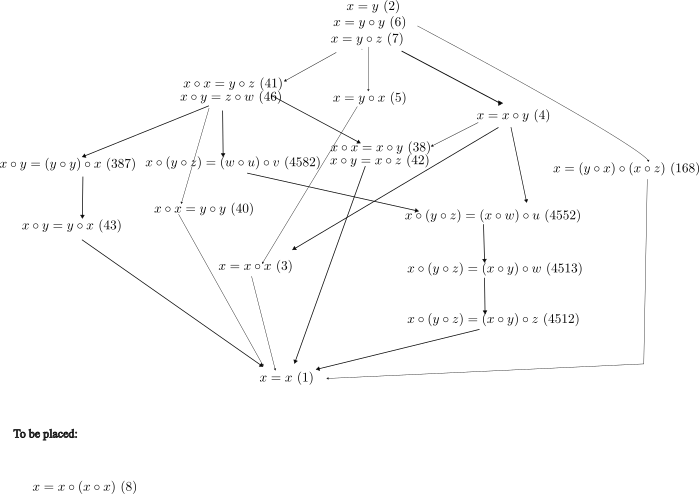
\includegraphics[width=0.5\linewidth]{../../images/implications.png}
  \caption{Implications between the above equations, displayed as a Hasse diagram.}
  \label{fig:implications}
\end{figure}


\begin{lemma}[Maximal element]\label{maximal}\uses{pre-order}\lean{Law.MagmaLaw.Equation1_maximal}\leanok The law $0  \formaleq  0$ is the maximal element in this pre-order.
\end{lemma}

\begin{proof} Trivial.
\end{proof}

\begin{lemma}[Minimal element]\label{minimal}\uses{pre-order}\lean{Law.MagmaLaw.Equation2_minimal}\leanok  The law $0  \formaleq  1$ is the minimal element in this pre-order.
\end{lemma}

\begin{proof} Trivial.
\end{proof}

Every magma $G$ has a \emph{reversal} $G^{\mathrm{op}}$, formed by by replacing the magma operation $\op$ with its opposite $\op^{\mathrm{op}}:(x,y) \mapsto y \op x$. There is a natural isomorphism between these magmas, which induces an involution $w \mapsto w^{\mathrm{op}}$ on words $w \in M_X$.  Every law $w  \formaleq  w'$ then has a \emph{dual} $w^{\mathrm{op}}  \formaleq  (w')^{\mathrm{op}}$.

For instance, the dual of the law $0 \op 1 = 0 \op 2$ is $1 \op 0 = 2 \op 0$, which after relabeling is $0 \op 1 = 2 \op 1$.  A list of equations and their duals can be found \href{https://github.com/teorth/equational_theories/blob/main/data/dual_equations.md}{here}.  Of the 4694 equations under consideration, 84 are self-dual, leaving 2305 pairs of dual equations.

The pre-ordering on laws has a duality symmetry:

\begin{lemma}[Duality of laws]\label{duality}\uses{pre-order}  If $w  \formaleq  w'$ implies $w''  \formaleq  w'''$, then $w^{\mathrm{op}}  \formaleq  (w')^{\mathrm{op}}$ implies $w''^{\mathrm{op}}  \formaleq  (w''')^{\mathrm{op}}$.
\end{lemma}

\begin{proof} This follows from the fact that a magma $G$ satisfies a law $w  \formaleq  w'$ if and only if $G^{\mathrm{op}}$ satisfies $w^{\mathrm{op}}  \formaleq  (w')^{\mathrm{op}}$.
\end{proof}

Some equational laws can be ``diagonalized'':

\begin{theorem}[Diagonalization]\label{diag}  An equational law of the form
  \begin{equation}\label{prediag} F(x_1,\dots,x_n) = G(y_1,\dots,y_m),
  \end{equation}
  where $x_1,\dots,x_n$ and $y_1,\dots,y_m$ are distinct elements of the alphabet, implies the diagonalized law
$$ F(x_1,\dots,x_n) = F(x'_1,\dots,x'_n).$$
where $x'_1,\dots,x'_n$ are distinct from $x_1,\dots,x_n$
In particular, if $G(y_1,\dots,y_m)$ can be viewed as a specialization of $F(x'_1,\dots,x'_n)$, then these two laws are equivalent.
\end{theorem}

\begin{proof}  From two applications of \eqref{prediag} one has
$$ F(x_1,\dots,x_n) = G(y_1,\dots,y_m)$$
and
$$ F(x'_1,\dots,x'_n) = G(y_1,\dots,y_m)$$
whence the claim.
\end{proof}

Thus for instance, Definition \ref{eq7} is equivalent to Definition \ref{eq2}.

\begin{theorem}[Laws implied by the constant law]\label{constant-impl}\uses{impl,eq46}  If $w, w'$ each have order at least one, then the law $w \formaleq w'$ is implied by the constant law (Definition \ref{eq46}).  If exactly one of $w, w'$ has order zero, and the law $w \formaleq w'$ is not implied by the constant law.
\end{theorem}

\begin{proof} Routine.
\end{proof}

\begin{theorem}[Criterion for implication]\label{variable-impl}\uses{impl}\lean{Law.MagmaLaw.SameCount.derive}\leanok  If $w \formaleq w'$ is such that every variable appears the same number of times in both $w$ and $w'$, and $w \formaleq w'$ implies another law $w'' \formaleq w'''$, then every variable appears the same number of times in both $w''$ and $w'''$.
\end{theorem}

\begin{proof} Consider the magma $\mathrm{MS}$ of multisets over an arbitrary set $A$ (which can be seen as finitely supported maps $A\rightarrow \N$), with the multiset addition law $+$.  By hypothesis, this magma obeys $w \formaleq w'$, and hence $w'' \formaleq w'''$, giving the claim by comparing the orders of the elements of $A$ appearing in $w''$ and $w'''$ in this magma.
\end{proof}
